\documentclass{article}
\usepackage[utf8]{inputenc}
\usepackage[spanish]{babel}
\usepackage{listings}
\usepackage{graphicx}
\graphicspath{ {images/} }
\usepackage{cite}

\begin{document}

\begin{titlepage}
    \begin{center}
        \vspace*{1cm}
            
        \Huge
        \textbf{Taller memoria}
            
        \vspace{0.5cm}
        \LARGE
        Informática 2
            
        \vspace{1.5cm}
            
        \textbf{Julián Mauricio Sánchez Ceballos}
         \newline 
            CC: 1001132830   
        \vfill
            
        \vspace{0.8cm}
            
        \Large
        Departamento de Ingeniería Electrónica y Telecomunicaciones\\
        Universidad de Antioquia\\
        Medellín\\
        Septiembre de 2020
            
    \end{center}
\end{titlepage}
\tableofcontents

\newpage
\section{Introducción}
Dentro del ámbito de la computación se encuentran elementos que debido a su importancia y su categórico papel se deben estudiar de manera profunda para el correcto conocimiento de la computación, la memoria del computador cumple con los requisitos de ser un elemento que debido a su importancia, se hace elemental el conocer su funcionamiento, en gran parte, para sacar el mayor provecho a este recurso. Para esto es necesario devolverse al siglo pasado y como dice Barceló: "Aunque los ordenadores han ido incorporando muchos perfeccionamientos técnicos, el principio que rige su funcionamiento se estableció hace ya más de cincuenta años. por el matemático John Von Neumann en su libro 'Primer esbozo de un informe sobre el EDVAC'(First draft of a report on the EDVAC, 1945)"\cite{barcelo}. Pues es en la Arquitectura Von Neumann en donde se define la funcionalidad de la memoria y su relación con el procesador que es el encargado de ejecutar cambios sobre los datos almacenados en la memoria y los periféricos de entrada y salida que son los encargados de recoger y mostrar los cambios hechos a los datos de la memoria respectivamente.\newline


Es por lo que el propósito de este documento es el estudio a fondo de la memoria, su funcionamientos, los tipos de memoria, las características, ventajas, capacidad y velocidad, con esto el entendimiento de la memoria darán una visión mas general sobre las ventajas de saber aprovechar este elemento en la computación, siendo de gran ayuda el entender esto para la tarea de crear algoritmos eficientes y saque provecho de la memoria. 
\newline

En el siguiente taller se resuelven cuestiones acerca de la memoria en base a una lectura previa del documento brindado por el profesor Augusto Enrique Salazar Ramirez Jimenez en su texto ''Como funciona la memoria de un computador''
\newpage
\section{Taller}

    \subsection{Defina que es la memoria del computador}
    La memoria es un componente en las computadoras que tiene como función conectar la unidad central de procesamiento y los elementos de entrada y salida, allí  la información de aplicaciones, instrucciones y datos es almacenada de manera temporal, a estos datos se les puede efectuar operaciones de lectura y escritura, para luego ser almacenados en el disco duro de nuevo, como existen tipos de memorias donde los datos se eliminan una vez se dejan de usar(volátiles) también están las memorias que guardan la información y los datos incluso después de apagarse el computador(no volátiles) la funcionalidad de ambas recurren al mismo propósito de almacenar información, lectura y escritura de datos, aunque su velocidad en estas dos ultimas funcionalidades puede variar según el tipo de memoria de la que se trate, puesto a los diferentes tipos de memoria estas tienen una jerarquía. \cite{Mano}
    
        \begin{figure}[h]
        \includegraphics[width=8cm]{jerarquia.jpg}
        \centering
        \caption{ejemplo de Jerarquía de la memoria}
        \label{fig:Jerarquia}
        \end{figure}   
     
     como se muestra en la figura \ref{fig:Jerarquia} las memorias tienen una Jerarquía, en este caso la jerarquía es de velocidad, entre más cerca está a la CPU, mas se acerca a la velocidad con la que trabaja este, al igual que entre más alejado este de la CPU más capacidad de almacenamiento tendrá.  
        
    \subsection{mencione los tipos de memoria que conoce y haga una pequeña descripción de cada tipo}
    En una computadora hay varios tipos de memoria como: 
    
        \subsubsection{Memoria Ram}
        ''Random Access Memory(memoria de acceso aleatorio) por sus siglas en ingles, es el tipo de memoria mas importante del computador y la mas usada.'' \cite{arquitectura} \newline

        Esta memoria compuesta de chips de memoria que a si vez se componen de transistores y capacitores se divide en celdas en donde se almacenan temporalmente los bits de información, esta memoria puede tener dos presentaciones una RAM dinámica que esta compuesta de capacitores que se vacían rápidamente de electrones que representan el 1 en el lenguaje binario por lo que es debido recargar constantemente estas celdas y la RAM estática que es está compuesta principalmente por cuatro o seis transistores en cada celda, logrando así que no sea necesario estar refrescando o recargando constantemente las celdas que representen un 1.
        
        \begin{figure}[h]
        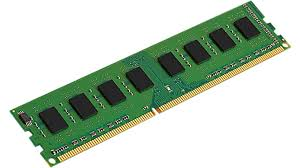
\includegraphics[width=4cm]{ram.jpg}
        \centering
        \caption{Memoria RAM}
        \label{fig:Memoria RAM}
        \end{figure}    
        
        la figura \ref{fig:Memoria RAM} muestra el aspecto de una memoria RAM y los componentes (placa de componentes, bancos de memoria, buses de conexión).
        
        \subsubsection{Memoria cache}
        Una memoria mucho mas rápida que la memoria RAM, se divide en tres niveles L1, L2 y L3, escritas desde el nivel con mas potencia hasta el menos potente y desde el mas pequeño al mas grande en almacenamiento respectivamente. ''Por ello, el caché L1 se integra, junto con la CPU, en un único circuito integrado, y se denomina caché interna, como en el procesador genérico. Pero el área  disponible en un circuito integrado es limitada.'' \cite{Mano}
        
        Es allí donde se lleva la información mas usada en el computador. Se encuentra en núcleo del computador y su principal problema es el costo de producción, al ser tan alto es poco viable incorporarlas en grandes cantidades en los computadores hogareños, sin embargo es la memoria mas rápida que se puede incorporar en un computador.   
        
        
        
        
        \subsubsection{Memoria virtual}
        Se trata de una porción de disco duro donde se almacena aplicaciones en ejecución y que no ocupan tanto espacio, estas aplicaciones están listas para ser usadas en cualquier momento sin ocupar espacios innecesarios en la memoria RAM, de esta manera se permite un uso más eficiente de la memoria RAM facilitando que se hagan procesos múltiples y ejecutar aplicaciones de manera simultanea.
        
        Entre algunas capacidades de esta memoria están;ejecutar programas sin necesidad de memoria física, simulación de RAM y extensión de su tamaño por medio del disco duro.\cite{gestion}  
        
        \subsubsection{memoria disco duro}
        la Memoria de Disco duro o memoria no volátil se encarga de guardar los datos que la memoria RAM elimina una vez se dejaron de usar, la capacidad de lectura  escritura es muchísima mas pequeña que la capacidad que tiene la memoria RAM, sin embargo la principal utilidad de esta memoria radica en su característica de no volátil permitiendo almacenar los datos y cambios que se hagan a los datos aun luego de apagar el computador, es importante decir que es desde aquí donde el bus de información toma los datos para ser llevados a la memoria RAM donde se ejecutan cambios sobre los datos originales. 
        
        \begin{figure}[h]
        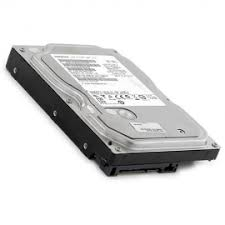
\includegraphics[width=4cm]{discoDuro.jpg}
        \centering
        \caption{Disco Duro}
        \label{fig:discoDuro}
        \end{figure}
        
        la Figura \ref{fig:discoDuro} muestra la apariencia de un disco duro, usualmente instalado en los computadores caseros 
        
        \subsubsection{Memorias Flash}
        Son memorias hechas a partir de del uso de semiconductores no volátiles y re-escribibles, útiles que permite la lectura y escritura de múltiples posiciones de memoria en la misma operación, esto otorga una gran velocidad de funcionamiento sobre las memorias tipo ROM. Una de sus ventajas más importantes es el bajo costo y su aumento de capacidad, además de su bajo consumo de energía y su portabilidad 
        
        \begin{figure}[h]
        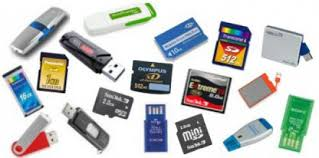
\includegraphics[width=4cm]{flash.jpg}
        \centering
        \caption{Memoria Flash}
        \label{fig:flash}
        \end{figure}
        
        La figura \ref{fig:flash} muestra las distintas formas de una memoria flash
    
    \subsection{describa la manera como se gestiona la memoria en un computador}
    La gestión de la memoria se hace a través de microprocesadores que saca la información o los datos y los lleva del disco duro a la memoria donde se  leen y se modifica a gusto del usuario, mediante operaciones lógicas que suceden dentro del procesador que es donde los cambios se generan, luego de terminar el proceso con los datos estos mismos microprocesadores llevan la información modificada a el disco duro mediante el bus de datos, en el disco duro los microprocesadores sobrescriben el mismo archivo, con esto se reemplaza por el archivo viejo por el nuevo, donde están los cambios que el usuario realizó. 
    El archivo es eliminado de la memoria RAM para evitar que ocupe espacio innecesario, con esto se puede asignar espacio a la memoria a otros procesos que necesiten, que igualmente lo liberaran cuando ya no lo requieran, de esta gestión se encarga el sistema operativo, ciertamente lo hace el administrados de memoria y su labor consiste en llevar el registro de las aplicaciones que necesitan memoria, la cantidad que necesitan y cuando ya no necesitan memoria.\cite{gestion}
 
    
    
    \subsection{¿Qué hace que una memoria sea más rápida que otra? ¿Por qué eso es importante?}
    la memoria del sistema tiene mas rapidez si la CPU tiene que esperar menos para acceder a los datos, o sea, la cantidad de latencia que tenga una memoria, este es el tiempo que transcurre entre la petición de la CPU y la respuesta de la memoria para enviar o recibir los datos que requiere la CPU. 
    
    Esta cuestión es importante debido a la importancia de la memoria dentro del funcionamiento de un computador, un computador con una memoria de buena calidad y más rápida podrá hacer trabajos mas exigentes y de maneras más rápidas, teniendo en cuenta la gran velocidad con la que la tecnología avanza y que cada vez los programas son mas exigentes, se manejan mucho mas datos, el tener una memoria rápida y con buena capacidad de almacenamiento se convierte en un tema de competitividad entre marcas, o empresas de programación que estén bien dotadas y proporcionalmente mas aptas a superar nuevos y mas exigentes retos que surgen en el mundo de la informática. 


\section{Conclusión} \label{conclulsion}
Desde la concepción de la arquitectura Von Neumann hasta nuestros días la memoria de un computador ha jugado un papel importante, convirtiéndose en un componente sumamente necesario de estudiar en cursos como este, donde el programar es intrínseco a la necesidad de utilizar los recursos que se brindan con la mayor eficacia posible, recursos mayormente gestionados por la memoria, dado que, por lo que pudimos ver es allí donde la computación se muestra en todo su esplendor, pues, es en la memoria donde los datos son almacenado, analizados, modificados, se leen y se sobrescriben, haciendo posible la información de la que incluso ahora mismo está siendo testigo al leer este documento. Frente a los ámbitos a analizar en una memoria podría resumirse en el tipo de memoria, su velocidad y capacidad de almacenamiento, la manera de como se gestiona la información allí. Comprender las características anteriormente mencionadas produce una  visión mas general de la computación y su funcionamiento desde los conceptos mas básicos, haciendo del programador una persona con capacidades y actitudes a la altura de crear programas que manejen de manera adecuada, provechosa y eficiente los recursos que le brindan los medios con los que trabaja.
\bibliographystyle{IEEEtran}
\bibliography{references}

\end{document}


